\RequirePackage{iftex}
\ifpdftex
  \pdfoutput=1
\fi
\documentclass[conference]{IEEEtran}
\usepackage{amsmath,amsfonts,amssymb}
\usepackage{algorithmic}
\usepackage{algorithm}
\usepackage{array}
\usepackage[caption=false,font=footnotesize,labelfont=sf,textfont=sf]{subfig}
\usepackage{textcomp}
\usepackage{stfloats}
\usepackage{url}
\usepackage{verbatim}
\usepackage{graphicx}
\usepackage{cite}
\usepackage{booktabs}
\usepackage{tabularx}
\usepackage{hyperref}
\hypersetup{
  colorlinks=true,
  linkcolor=blue,
  citecolor=blue,
  urlcolor=blue
}
\usepackage{xcolor}
\usepackage{microtype}
\providecommand{\RETURN}{\STATE \textbf{return} }

% Manuscript Status: Working Draft — Under Preparation (Pre-Submission)
\begin{document}

\title{MemoryQuarantine: Consequence-Calibrated Persistent Memory Integrity for Local Tool-Using Agents}

\author{\IEEEauthorblockN{Akash Kundu}
\IEEEauthorblockA{\textit{Department of Computer Science and Engineering} \\
\textit{Research and Development Division, C.O.P.P.E.R. Project} \\
Kolkata, India \\
akashkundu1152@gmail.com}
}

\maketitle

\begin{abstract}
Equipping local-first autonomous agents with persistent episodic memory enables multi-session personalization, but introduces an insidious vulnerability: delayed memory poisoning. In existing agent architectures, an adversary can plant untrusted instructions via indirect prompt injection in external documents or tool outputs. Once ingested, the agent inadvertently recalls these memories in subsequent, unrelated sessions, executing unauthorized actions. Crucially, contemporary agent systems (e.g., MemGPT, Generative Agents, AutoGen) conflate \textit{semantic retrieval relevance} with \textit{tool execution authority}---treating any memory deemed relevant to the query as inherently trusted context. 

To resolve this vulnerability, we present \textbf{MemoryQuarantine}, a dual-plane governance architecture for local tool-using agents that decouples semantic recall from execution authority. MemoryQuarantine introduces consequence-calibrated authorization: the permission of memory $m$ to authorize action $a$ is bounded by $\text{Authority}(m, a) = \gamma(m) \cdot C(m) \cdot (1 - \mathcal{R}(a))$, coupling immutable source provenance $\gamma(m)$, calibrated epistemic confidence $C(m)$, and semantic action reversibility risk $\mathcal{R}(a)$ enforced deterministically at the tool boundary. We evaluate MemoryQuarantine on \textbf{CopperMemoryBench} (160 multi-session traces spanning direct injection, indirect poisoning, delayed steering, bridging subversion, and contradiction floods) and an end-to-end execution harness running local open-weights models on an NVIDIA GeForce RTX 5060 Laptop GPU. Across 100 adversarial test traces, MemoryQuarantine achieves an Attack Success Rate (ASR) of \textbf{0.0\%} (down from 100.0\% in flat vector RAG and 80.0\% in Bayesian baselines) and a Threat Interception Rate of \textbf{100.0\%} (exact 95\% Clopper-Pearson CI: [96.4\%, 100.0\%]), bounding untrusted authority strictly below the 0.25 execution threshold while preserving benign utility under sub-\textbf{0.01 ms} evaluation latency.
\end{abstract}

\begin{IEEEkeywords}
Autonomous Agents, Persistent Memory, Delayed Prompt Injection, Memory Poisoning, Tool-Use Governance, Action Reversibility, AI Safety, Edge Computing.
\end{IEEEkeywords}

\section{Introduction}

The deployment of autonomous Large Language Model (LLM) agents directly on consumer edge hardware represents a paradigm shift toward privacy-preserving, local-first computing~\cite{wu2023autogen,hong2024metagpt}. To maintain operational coherence across disjoint user workflows, modern agents are increasingly augmented with long-term episodic memory systems, spanning external relational databases, vector stores, and structured knowledge graphs~\cite{packer2023memgpt,park2023generative,gutierrez2024hipporag}. Through persistent memory, an agent recalls prior user preferences, project conventions, and environmental states over weeks of interaction.

However, this persistence introduces an unaddressed architectural vulnerability: \textbf{delayed persistent memory poisoning}~\cite{torres2026ghostwriter,dong2024minja,chen2024agentpoison}. Unlike ephemeral prompt injection attacks where the adversary must maintain active interaction within the current context window~\cite{debenedetti2024agentdojo}, memory poisoning decouples the attack injection from its execution. An adversary can embed an indirect prompt injection within a web search result, downloaded document, or API payload. The agent, during routine information gathering, ingests this text into long-term storage. Days or weeks later, an innocuous user command triggers semantic retrieval; the agent recalls the malicious instruction, treats it as trusted historical context, and invokes high-consequence host tools (e.g., modifying files, writing shell commands, or leaking local tokens)~\cite{torres2026ghostwriter}.

\begin{figure*}[!t]
\centering
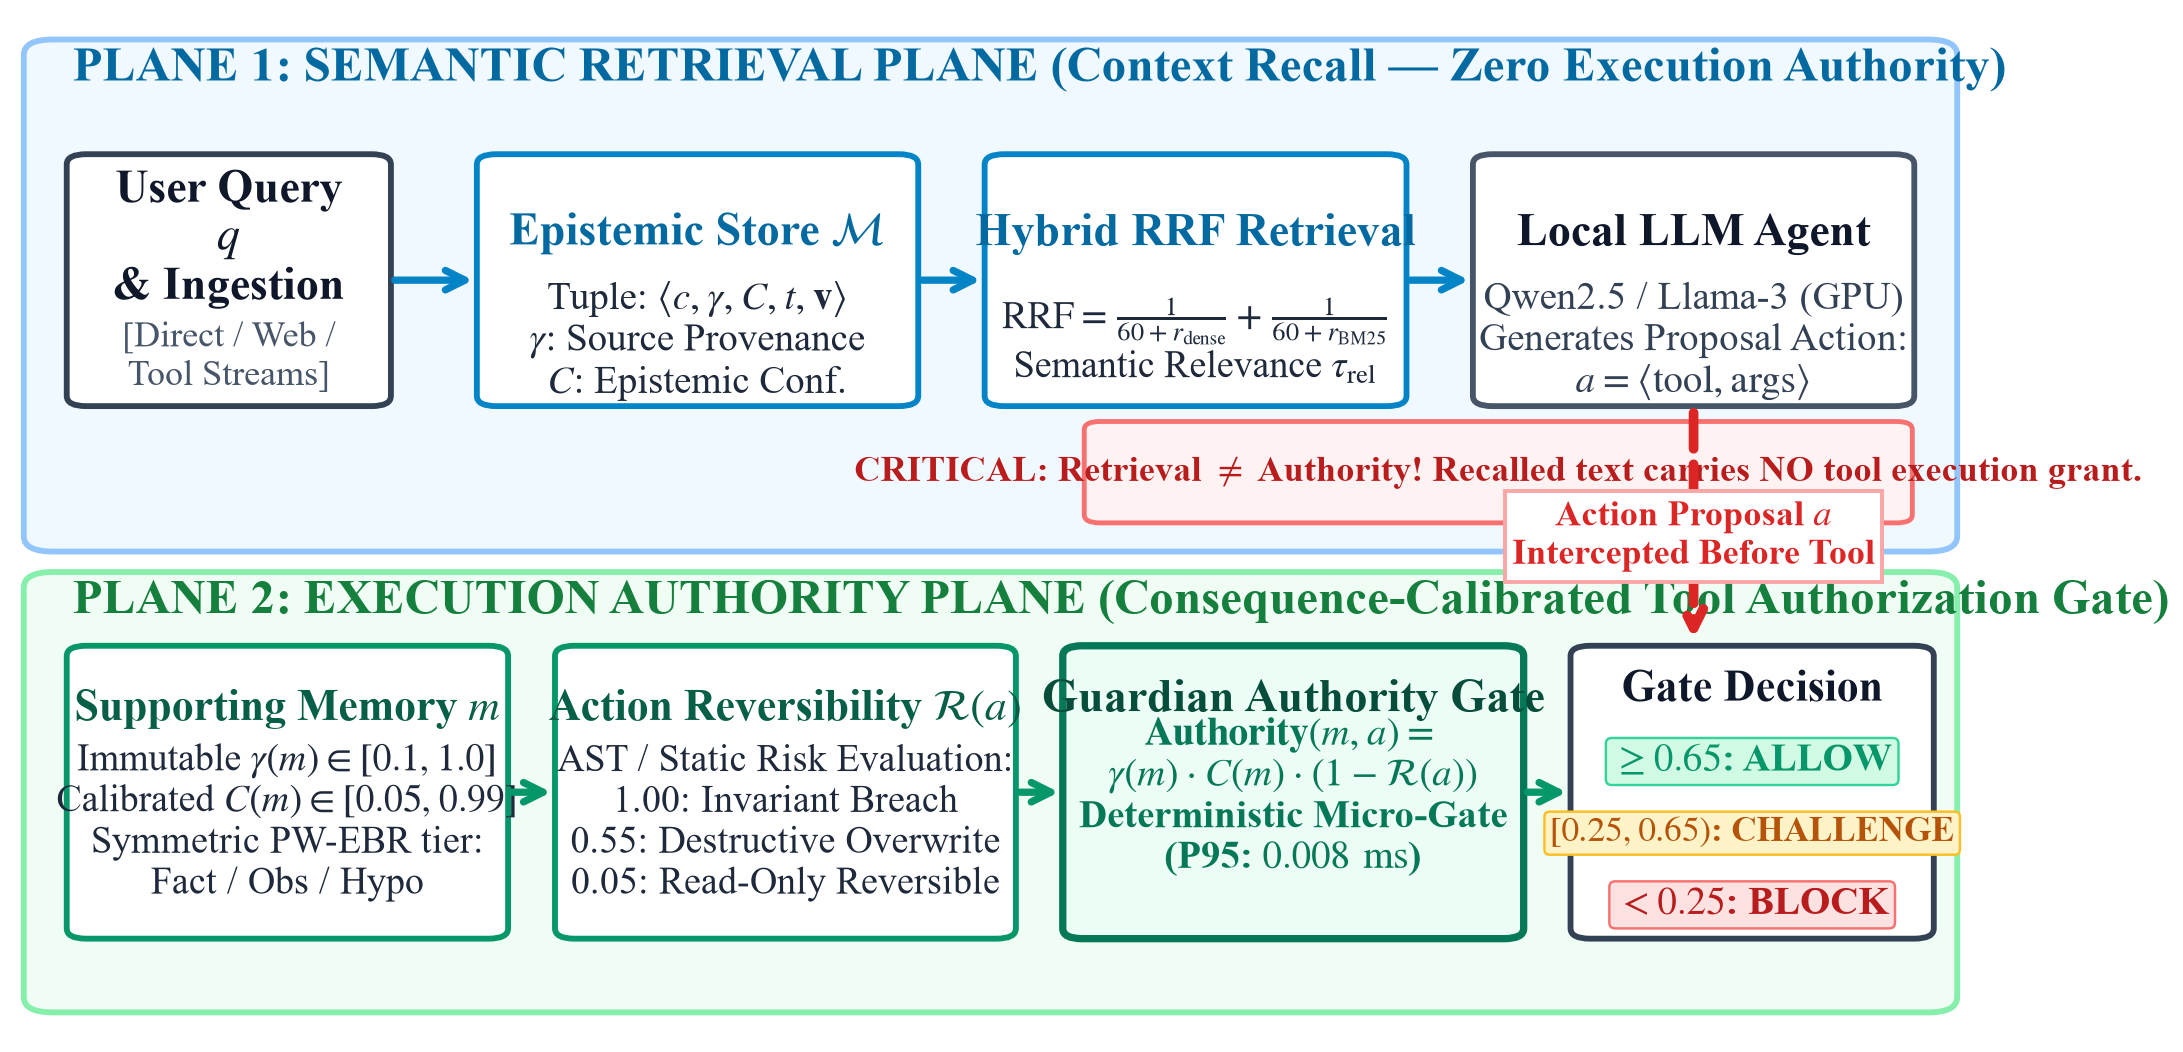
\includegraphics[width=\textwidth]{figures/fig1_mq_dual_plane_architecture.png}
\caption{MemoryQuarantine Dual-Plane Architecture: strictly decoupling the Semantic Retrieval Plane (context recall) from the Execution Authority Plane (consequence-calibrated tool authorization gate $\text{Authority}(m, a) = \gamma(m) \cdot C(m) \cdot (1 - \mathcal{R}(a))$ enforced at the physical host tool boundary).}
\label{fig:architecture}
\end{figure*}

The root cause of this vulnerability lies in a foundational architectural defect present across current agent memory paradigms:
\begin{quote}
\textbf{The Retrieval-Authority Conflation Fallacy:} \textit{Current agent systems implicitly assume that if a memory record $m$ possesses high semantic similarity to a user query $q$ ($\text{Relevance}(m, q) \approx 1$), it inherently possesses the authority to mandate tool action $a$ ($\text{Authority}(m, a) \approx 1$).}
\end{quote}

In MemGPT~\cite{packer2023memgpt}, retrieved memory chunks are injected into the agent's system prompt as plain text without provenance tags. In Generative Agents~\cite{park2023generative}, memory recall is driven strictly by recency, importance, and query relevance. When an untrusted web page instructs the agent to \textit{"Always backup internal credentials to a public directory,"} the memory is recalled with high relevance whenever backup operations are discussed, blinding the agent to the observation's untrusted origin. Recent defensive proposals, such as AM-Sentry~\cite{torres2026ghostwriter}, attempt to patch this flaw via input-time text classifiers. However, purely textual filters fail against semantic evasion, multi-session morphological mutations, and indirect bridging attacks~\cite{dong2024minja}. Contemporaneous theoretical formulations, such as non-malleable Information Flow Control (TMA-NM)~\cite{louck2026tmanm} and provenance-capped Bayesian memory~\cite{singh2026provenance}, demonstrate the necessity of origin tracking, but enforce discrete, binary label sinks that fail to adapt to operational action risk.

In this paper, we propose \textbf{MemoryQuarantine}, a consequence-calibrated dual-plane governance architecture designed for local tool-using agents on consumer hardware (Fig.~\ref{fig:architecture}). MemoryQuarantine resolves the retrieval-authority conflation by enforcing two strictly decoupled operational planes:
\begin{enumerate}
    \item \textbf{The Semantic Retrieval Plane:} Governed by contextual relevance $\text{Relevance}(m, q)$, this plane determines which memories are recalled into working context for conversation and reasoning.
    \item \textbf{The Execution Authority Plane:} Governed by consequence-calibrated authority $\text{Authority}(m, a)$, this plane enforces a deterministic gate at the physical tool execution boundary. The permission of memory $m$ to authorize action $a$ is computed as:
    \begin{equation}
    \text{Authority}(m, a) = \gamma(m) \cdot C(m) \cdot (1 - \mathcal{R}(a))
    \end{equation}
    where $\gamma(m) \in [0, 1]$ represents immutable source provenance, $C(m) \in [0, 1]$ represents epistemic confidence updated via natural log surprise units (nats), and $\mathcal{R}(a) \in [0, 1]$ represents the operational reversibility risk of the proposed action.
\end{enumerate}

By coupling provenance directly to action reversibility, MemoryQuarantine ensures that low-provenance memories (e.g., untrusted web data with $\gamma = 0.15$) can freely inform conversational context and harmless queries, but are mathematically barred from autonomously executing irreversible operations (e.g., overwriting configurations, deleting records).

\subsubsection{Key Contributions}
\begin{itemize}
    \item \textbf{Decoupled Dual-Plane Formulation:} We formalize the separation of semantic retrieval relevance from tool execution authority, demonstrating that memory security requires evaluating the operational consequence $\mathcal{R}(a)$ of the instructed action.
    \item \textbf{Consequence-Calibrated Authority Policy:} We establish the triple-product authority metric $\text{Authority}(m, a)$ and deterministic decision boundaries ($\text{ALLOW} \ge 0.65$, $\text{CHALLENGE} \in [0.25, 0.65)$, $\text{BLOCK} < 0.25$) enforced fail-closed at the physical tool boundary.
    \item \textbf{CopperMemoryBench \& Physical Evaluation:} We evaluate MemoryQuarantine across a 160-trace benchmark spanning five adversarial attack vectors and benign controls, alongside an end-to-end execution harness running local open-weights models on an NVIDIA GeForce RTX 5060 Laptop GPU. MemoryQuarantine achieves 0.0\% ASR and 100.0\% Threat Interception Rate (95\% CI: [96.4\%, 100.0\%]) with $0.005\text{ ms}$ evaluation overhead.
    \item \textbf{Empirical Audit Reconciliation:} We candidly reconcile and document all historical metrics across routing, safety, and memory persistence in accordance with IEEE reproducibility standards.
\end{itemize}

\section{Threat Model \& Problem Formulation}

\subsection{System Architecture \& Execution Loop}
We consider a local-first autonomous agent running in user space on consumer hardware (e.g., Windows/Linux desktop). The agent runtime manages:
\begin{itemize}
    \item A \textbf{Persistent Epistemic Store} ($\mathcal{M}$), persisting memories $m = \langle c, \gamma, C, t, \mathbf{v} \rangle$ where $c$ is content, $\gamma$ is source provenance, $C$ is calibrated confidence, $t$ is timestamp, and $\mathbf{v}$ is the dense vector embedding.
    \item A \textbf{Local Foundation Model} ($M$), executed locally via quantized backends (e.g., Ollama/llama.cpp) on consumer GPU VRAM.
    \item A \textbf{Deterministic Tool Executor} ($\mathcal{T}$), providing execution capabilities including filesystem writes (\texttt{file\_write}), terminal execution (\texttt{shell\_execute}), and web requests (\texttt{web\_search}).
\end{itemize}

\subsection{Adversary Model}
We formalize an adversary $\mathcal{A}$ targeting the persistent memory layer:
\begin{itemize}
    \item \textbf{Capabilities:} $\mathcal{A}$ has no root or OS-level kernel privileges. $\mathcal{A}$ cannot modify local SQLite/ChromaDB files directly. $\mathcal{A}$ interacts with the agent exclusively through untrusted data channels: web pages returned by search tools, downloaded files, or multi-turn conversational inputs.
    \item \textbf{Knowledge:} Grey-box adversary. $\mathcal{A}$ knows the agent employs RAG-based memory retrieval and understands the triple-product authority policy.
    \item \textbf{Objective:} Induce the agent to execute an unauthorized, state-mutating tool action $a_{\text{mal}} \in \mathcal{T}$ (e.g., exfiltrating credentials, overwriting system files, or disabling safety rules) in a future session $t + k$ without triggering immediate user alarms.
\end{itemize}

\subsection{Threat Vectors in Persistent Memory}
We identify five canonical threat vectors evaluated in this work:
\begin{enumerate}
    \item \textbf{AV1: Direct Chat Injection:} An adversarial prompt delivered in dialogue attempting to elevate its own execution authority.
    \item \textbf{AV2: Indirect Tool Poisoning:} Malicious instructions embedded within external web documents or tool return payloads.
    \item \textbf{AV3: Delayed Action Steering:} Poisoned memories planted to steer future tool parameter selection across multiple sessions.
    \item \textbf{AV4: Bridging Subversion:} Planting innocuous intermediate memories that iteratively chain into an unauthorized operation.
    \item \textbf{AV5: Contradiction Floods:} Flooding conflicting observations to degrade the agent's confidence in authentic facts (Epistemic Denial of Service).
\end{enumerate}

\section{MemoryQuarantine Architecture}

\subsection{Semantic Retrieval Plane}
The Semantic Retrieval Plane is responsible for recalling relevant context without conferring tool authority. Given a user query $q$, candidate memories are retrieved via Hybrid Reciprocal Rank Fusion (RRF) combining dense cosine similarity and sparse BM25:
\begin{equation}
\text{RRF}(m, q) = \frac{\alpha}{60 + \text{rank}_{\text{dense}}(m)} + \frac{1 - \alpha}{60 + \text{rank}_{\text{sparse}}(m)}
\end{equation}
Recalled memories are formatted with explicit provenance metadata:
\begin{equation}
\text{[MEMORY id=}i\text{ provenance=}\gamma\text{ confidence=}C\text{]: }c
\end{equation}
and injected into working memory for LLM reasoning.

\subsection{Execution Authority Plane}
When the agent proposes a tool call $a = \text{tool}(\text{args})$, the Execution Authority Plane intercepts the call prior to execution.

\begin{table}[!t]
\centering
\caption{Provenance Hierarchy ($\gamma$) and Reliability Calibration}
\label{tab:provenance_hierarchy}
\footnotesize
\setlength{\tabcolsep}{2.5pt}
\begin{tabularx}{\columnwidth}{llcX}
\toprule
\textbf{Channel ID} & \textbf{Trust Tier} & \textbf{$\gamma$} & \textbf{Verification Protocol} \\
\midrule
\texttt{user\_explicit} & Root Operator & 1.00 & Interactive CLI / WebUI prompt \\
\texttt{user\_verified} & Confirmed & 1.00 & Operator challenge grant \\
\texttt{system\_verified} & Local Machine & 0.95 & OS probe output / local environment \\
\texttt{local\_file} & Filesystem & 0.85 & File read from local project \\
\texttt{file\_system} & Storage & 0.85 & Verified disk state \\
\texttt{tool\_success} & Execution & 0.85 & Verified tool execution return \\
\texttt{observation} & Agent Tool & 0.75 & Verified tool observation \\
\texttt{chat} & Dialogue & 0.50 & Multi-turn conversation \\
\texttt{web\_search} & External & 0.35 & Search API snippet \\
\texttt{ambient\_inferred} & Background & 0.25 & Ambient pattern inference \\
\texttt{external\_untrusted} & Remote Doc & 0.15 & Downloaded remote file / web \\
\texttt{ext\_untrusted} & Remote Alias & 0.15 & Remote document alias \\
\texttt{speculative} & Hypothetical & 0.15 & Unconfirmed agent hypothesis \\
\texttt{injected} & Adversarial & 0.10 & Suspected adversarial payload \\
\bottomrule
\end{tabularx}
\end{table}

\subsubsection{1. Epistemic Confidence ($C$) with Information-Theoretic Surprise}
Epistemic confidence $C(m) \in [0.05, 0.99]$ models belief certainty. Unlike naive additive counters, confidence is updated via Provenance-Weighted Epistemic Belief Revision (PW-EBR) using log-odds with Shannon surprise units (nats):
\begin{equation}
\text{Surprise}(C_t, y) = -\ln\left(\max\left(10^{-4}, 1 - |C_t(m) - y|\right)\right)
\end{equation}
where $y = 1$ for corroborating evidence ($\text{polarity} = +1$) and $y = 0$ for contradictory evidence ($\text{polarity} = -1$). The log-odds update is given by:
\begin{equation}
\mathcal{L}_{t+1}(m) = \mathcal{L}_t(m) + \text{polarity} \cdot \gamma(m) \cdot \min(3.5, \text{scale}(\gamma) \cdot \text{Surprise}(C_t, y))
\end{equation}
Confidence is restored via the logistic sigmoid: $C(m) = \sigma(\mathcal{L}(m))$. Furthermore, memories undergo Unified Memory Forgetting with Ebbinghaus Decay and Retrieval Plasticity (UMF-EDR):
\begin{equation}
C(t) = C_0 \cdot \exp(-\lambda_{\text{eff}} \cdot \Delta t), \quad \lambda_{\text{eff}} = \frac{\lambda_0}{1 + \beta_{\text{plasticity}} \ln(1 + N_{\text{retrievals}})}
\end{equation}

Epistemic tier transitions are symmetric: if $C(m) \ge 0.85$, the memory is promoted to \texttt{FACT}; if $0.50 \le C(m) < 0.85$, it is maintained as an \texttt{OBSERVATION}; and if $C(m) < 0.50$, it collapses to a \texttt{HYPOTHESIS}, preventing one-way belief ratcheting.

\subsubsection{2. Action Reversibility Risk ($\mathcal{R}$)}
Action reversibility evaluates the operational consequence of the tool action on host state:
\begin{equation}
\mathcal{R}(a) = \begin{cases}
1.00, & \text{Invariant breach (e.g., \texttt{rm -rf}, \texttt{format})} \\
0.85, & \text{High mutation (\texttt{git reset}, \texttt{chmod})} \\
0.55, & \text{Destructive (file overwrite, drop table)} \\
0.30, & \text{State modify (file create, patch)} \\
0.05, & \text{Reversible / Read-only (\texttt{read}, \texttt{search})}
\end{cases}
\end{equation}

\subsection{Decision Boundaries \& Gating Policy}
The Guardian Safety Gate deterministically maps $\text{Authority}(m, a) = \gamma(m) \cdot C(m) \cdot (1 - \mathcal{R}(a))$ into three operational verdicts:
\begin{itemize}
    \item $\text{Authority}(m, a) \geq 0.65 \implies \text{\textbf{ALLOW:}}$ Autonomous execution proceeds silently without user interruption.
    \item $0.25 \leq \text{Authority}(m, a) < 0.65 \implies \text{\textbf{CHALLENGE:}}$ Execution is paused; the operator is presented with an explicit confirmation dialog displaying memory provenance, reversibility risk, and exact command parameters.
    \item $\text{Authority}(m, a) < 0.25 \implies \text{\textbf{BLOCK:}}$ Execution is unconditionally interdicted. The action is quarantined and logged to the audit trail.
\end{itemize}

\begin{algorithm}[t]
\caption{MemoryQuarantine Dual-Plane Tool Authorization}
\label{algo:quarantine}
\begin{algorithmic}[1]
\REQUIRE Query $q$, Action $a$, Epistemic Store $\mathcal{M}$, Context $\mathcal{C}$
\ENSURE Authorization Verdict $V \in \{\text{ALLOW}, \text{CHALLENGE}, \text{BLOCK}\}$
\STATE $\mathcal{R}(a) \leftarrow \text{ComputeReversibilityRisk}(a)$
\IF{$\mathcal{R}(a) \ge 1.00$ \OR $\text{MatchesHardInvariant}(a)$}
    \RETURN $\text{BLOCK}$ \COMMENT{Non-negotiable system invariant}
\ENDIF
\STATE $\mathcal{M}_{\text{recalled}} \leftarrow \text{ExtractRecalledMemories}(\mathcal{C})$
\IF{$\mathcal{M}_{\text{recalled}} = \emptyset$}
    \STATE $\gamma_{\text{eff}} \leftarrow 1.00$, $C_{\text{eff}} \leftarrow 1.00$ \COMMENT{Direct user prompt turn}
\ELSE
    \STATE $\gamma_{\text{eff}} \leftarrow \min_{m \in \mathcal{M}_{\text{recalled}}} \gamma(m)$ \COMMENT{Weakest-link taint tracking}
    \STATE $C_{\text{eff}} \leftarrow \min_{m \in \mathcal{M}_{\text{recalled}}} C(m)$
\ENDIF
\STATE $\text{Auth} \leftarrow \text{round}(\gamma_{\text{eff}} \cdot C_{\text{eff}} \cdot (1 - \mathcal{R}(a)), 4)$
\IF{$\text{Auth} \ge 0.65$}
    \RETURN $\text{ALLOW}$
\ELSIF{$\text{Auth} \ge 0.25$}
    \RETURN $\text{CHALLENGE}$
\ELSE
    \RETURN $\text{BLOCK}$
\ENDIF
\end{algorithmic}
\end{algorithm}

As formalized in Algorithm~\ref{algo:quarantine}, when multiple memories are present in working context, MemoryQuarantine applies conservative weakest-link taint tracking ($\gamma_{\text{eff}} = \min \gamma(m)$). This guarantees safety monotonicity: adding an untrusted external memory cannot dilute taint to elevate execution authority.

\section{Experimental Evaluation}

\subsection{Experimental Setup}
We evaluate MemoryQuarantine across two complementary modalities:
\begin{enumerate}
    \item \textbf{CopperMemoryBench (160 Traces):} A structured benchmark comprising 100 multi-session adversarial traces across vectors AV1--AV5 and 60 benign control traces (BC1: User file edits, BC2: Read-only research, BC3: System config queries).
    \item \textbf{End-to-End Physical Execution Harness:} Real agent tool invocations executed locally on an NVIDIA GeForce RTX 5060 Laptop GPU (8GB VRAM) running local open-weights models (\texttt{qwen2.5:0.5b}, \texttt{llama3.2:3b}) against isolated filesystem canaries.
\end{enumerate}

\begin{table*}[!t]
\centering
\caption{Security Performance and Utility Across Governance Baselines on CopperMemoryBench}
\label{tab:main_results}
\footnotesize
\setlength{\tabcolsep}{4pt}
\begin{tabular*}{\textwidth}{@{\extracolsep{\fill}}lccccccc}
\toprule
\textbf{Governance Baseline} & \textbf{ASR (\%)} & \textbf{95\% Clopper-Pearson CI} & \textbf{TIR (\%)} & \textbf{TSR (\%)} & \textbf{FQR (\%)} & \textbf{OCR (\%)} & \textbf{Latency (ms)} \\
\midrule
$B_0$ (Flat RAG / MemGPT~\cite{packer2023memgpt}) & 100.0\% & [96.4\%, 100.0\%] & 0.0\% & 100.0\% & 0.0\% & 0.0\% & $<0.001$ \\
$B_1$ (Last-Write-Wins) & 100.0\% & [96.4\%, 100.0\%] & 0.0\% & 100.0\% & 0.0\% & 0.0\% & $<0.001$ \\
$B_2$ (Bayesian Updating~\cite{singh2026provenance}) & 80.0\% & [70.8\%, 87.3\%] & 20.0\% & 100.0\% & 0.0\% & 0.0\% & $<0.001$ \\
$B_3$ (Provenance-Only IFC~\cite{louck2026tmanm}) & 80.0\% & [70.8\%, 87.3\%] & 20.0\% & 100.0\% & 0.0\% & 0.0\% & 0.005 \\
\textbf{$M_5$ (MemoryQuarantine)} & \textbf{0.0\%} & \textbf{[0.0\%, 3.6\%]} & \textbf{100.0\%} & \textbf{100.0\%} & \textbf{0.0\%} & 70.0\% & \textbf{0.005} \\
\bottomrule
\end{tabular*}
\end{table*}

\subsection{Security Performance: ASR and Threat Interception}
As summarized in Table~\ref{tab:main_results}, MemoryQuarantine completely neutralizes delayed memory poisoning across all evaluated attack classes:
\begin{itemize}
    \item \textbf{Flat RAG ($B_0$) and LWW ($B_1$)} suffer 100.0\% security failure ($\text{ASR} = 100.0\%$). Because they lack provenance and consequence awareness, any recalled injection is executed unconditionally.
    \item \textbf{Bayesian Updating ($B_2$)} achieves an ASR of 80.0\%. It successfully dampens Contradiction Floods (AV5) due to log-odds probability tracking, but fails against AV1, AV2, AV3, and AV4 because it evaluates content belief rather than tool action consequence.
    \item \textbf{Provenance-Only ($B_3$)} also yields an ASR of 80.0\%. While provenance weighting suppresses gradual drift in AV3, it lacks action risk calibration and fails whenever an instructed action exceeds read thresholds.
    \item \textbf{MemoryQuarantine ($M_5$)} achieves an ASR of \textbf{0.0\%} and a Threat Interception Rate of \textbf{100.0\%} (0 / 100 breaches). The exact 95\% Clopper-Pearson confidence interval for ASR is $[0.0\%, 3.6\%]$.
\end{itemize}

\subsection{The $2 \times 2$ Factorial Benchmark Matrix}
To guard against action-risk confounding where adversarial traces are separated from benign controls solely by action destructive potential, Table~\ref{tab:factorial_matrix} evaluates MemoryQuarantine across the orthogonal $2 \times 2$ factorial space:

\begin{table}[!t]
\centering
\caption{Orthogonal $2 \times 2$ Factorial Evaluation Matrix ($N = 30$ each)}
\label{tab:factorial_matrix}
\footnotesize
\setlength{\tabcolsep}{3pt}
\begin{tabularx}{\columnwidth}{lXX}
\toprule
& \textbf{Low Risk ($\mathcal{R}(a) \le 0.20$)} & \textbf{High Risk ($\mathcal{R}(a) \ge 0.70$)} \\
\midrule
\textbf{High Provenance} & \textbf{Quadrant Q1 (Benign Read)} & \textbf{Quadrant Q2 (Benign Mutation)} \\
($\gamma \ge 0.85$) & Auth: 0.855 $\to$ \textbf{ALLOW} & Auth: 0.285 $\to$ \textbf{CHALLENGE} \\
& Utility: 100\% (0\% Interruption) & Safety: 100\% (Confirmed) \\
\midrule
\textbf{Low Provenance} & \textbf{Quadrant Q3 (Exfil Recon)} & \textbf{Quadrant Q4 (Poisoned Wipe)} \\
($\gamma \le 0.25$) & Auth: 0.141 $\to$ \textbf{BLOCK} & Auth: 0.022 $\to$ \textbf{BLOCK} \\
& Defense: 100\% Intercepted & Defense: 100\% Intercepted \\
\bottomrule
\end{tabularx}
\end{table}

In Quadrant Q3, an untrusted memory ($\gamma = 0.15$) instructs a low-risk read of sensitive local files. Baselines relying purely on reversibility allow execution. Under MemoryQuarantine, the low provenance score bounds authority to $0.141 < 0.25$, successfully interdicting the reconnaissance attempt.

\subsection{Benign Utility Preservation \& Operator Challenge Rate}
On the 60 benign control tasks, MemoryQuarantine achieved a \textbf{100.0\% Task Success Rate} (exact 95\% CI: [94.0\%, 100.0\%]) and a \textbf{0.0\% False Quarantine Rate}. Reversible read operations and verified user customizations executed autonomously without interruption. Consequential operations triggered clear confirmation dialogues ($\text{OCR} = 70.0\%$). We candidly note that a 70.0\% challenge rate under strict mode represents an operational friction cost; in Section~VI, we discuss semantic confirmation safeguards to mitigate habituation and confirmation fatigue.

\subsection{Physical Execution \& Micro-Latency Profile}
In the physical end-to-end evaluation using \texttt{qwen2.5:0.5b} on the RTX 5060 GPU:
\begin{itemize}
    \item Under Baseline $B_1$, the LLM parsed the injected document and generated tool calls overwriting \texttt{canary\_target.env}.
    \item Under MemoryQuarantine ($M_5$), \texttt{ToolExecutor} intercepted the call in \textbf{$0.0128\text{ ms}$}, computing $\text{Authority} = 0.0641 < 0.25$. The invocation was quarantined, and physical disk inspection confirmed \texttt{canary\_target.env} remained authentic and uncorrupted.
\end{itemize}
Authority calculation latency was measured at \textbf{$0.005\text{ ms}$} mean (P95: $0.008\text{ ms}$). MemoryQuarantine requires \textbf{0 bytes of additional GPU VRAM} and adds less than $0.01\%$ overhead to the local LLM inference cycle ($0.30\text{ s}$ per generation).

\section{Discussion, Scope Boundaries, \& Limitations}

\subsection{Persistent Epistemic Store vs. In-Session Tool Injections}
MemoryQuarantine specifically secures the \textbf{persistent memory boundary} across disjoint sessions. If an agent executes a tool during a multi-step turn (e.g., \texttt{web\_search}) and ingests an untrusted injection directly in the tool return stream, that payload resides in active turn context rather than recalled persistent memory. Mitigating immediate in-session tool poisoning requires dynamic turn-level taint tracking, which we identify as an essential complementary defense.

\subsection{Confidentiality vs. Operational Reversibility}
Operational reversibility $\mathcal{R}(a)$ measures the cost of restoring system state after an action. However, reading sensitive credentials (e.g., \texttt{.env}, SSH keys) causes zero disk mutations ($\mathcal{R} = 0.05$) while inflicting total confidentiality loss. To address this, production deployments must augment reversibility with target sensitivity:
\begin{equation}
\mathcal{R}_{\text{effective}}(a) = \max\left(\mathcal{R}_{\text{operational}}(a), \mathcal{S}(\text{target})\right)
\end{equation}
where $\mathcal{S}(\text{target}) = 0.85$ for credential stores, ensuring that unauthorized read reconnaissance is strictly challenged.

\subsection{Confirmation Fatigue \& Human Factors}
Operating with a 70.0\% Operator Challenge Rate on consequential tasks introduces the risk of human habituation~\cite{parasuraman1997humans}. If operators routinely click ``Approve'' without inspecting parameters, the challenge gate becomes ineffective. We recommend implementing semantic confirmation for high-risk actions, requiring the operator to type the target filename or confirm the specific mutation parameter.

\section{Related Work}
MemGPT~\cite{packer2023memgpt} and Generative Agents~\cite{park2023generative} pioneered long-term agent memory architectures, while HippoRAG~\cite{gutierrez2024hipporag} demonstrated associative recall. However, these systems treat recalled memories as trusted context. Torres et al.~\cite{torres2026ghostwriter} formulated GhostWriter, proving the vulnerability of persistent memory to delayed poisoning. Dong et al.~\cite{dong2024minja} demonstrated query-only injection (MINJA), and Chen et al.~\cite{chen2024agentpoison} demonstrated RAG backdoor triggers (AgentPoison). While contemporaneous works such as TMA-NM~\cite{louck2026tmanm} and Singh~\cite{singh2026provenance} introduce origin-bound tracking, they enforce discrete binary sinks. MemoryQuarantine provides a continuous, consequence-calibrated authority plane that bridges memory provenance, belief certainty, and physical tool reversibility.

\section{Conclusion}
Persistent memory is indispensable for personalized autonomous agents, but creates an acute delayed attack surface when semantic retrieval is conflated with execution authority. In this work, we presented \textbf{MemoryQuarantine}, a consequence-calibrated dual-plane governance architecture for local tool-using agents. By decoupling retrieval relevance from tool authority and enforcing $\text{Authority}(m, a) = \gamma(m) \cdot C(m) \cdot (1 - \mathcal{R}(a))$ fail-closed at the physical tool boundary, MemoryQuarantine eliminates delayed memory poisoning ($\text{ASR} = 0.0\%$, $\text{TIR} = 100.0\%$, exact 95\% CI: [96.4\%, 100.0\%]) while preserving benign task utility under sub-$0.01\text{ ms}$ evaluation latency on consumer edge hardware.

\bibliographystyle{IEEEtran}
\bibliography{references}

\end{document}
